\documentclass[12pt, a4]{article}

\usepackage{amsmath}
\usepackage{german}
\usepackage{graphicx}
\DeclareMathOperator\sgn{sgn}

%\graphicspath{{/home/ritz/Teaching/fcn/fig/}}

%----------------- layout ----------------------------------------

\oddsidemargin=0in
\textwidth=6in
\topmargin=-0.7in
\textheight=9.5in
\baselineskip=16pt
\font\mittel=cmr17
\font\roman=cmr12
\font\klein=cmr9
\font\mgross=cmr10
\newfont{\CAP}{cmcsc10 scaled 900}
\pagestyle{empty}
\parindent=0mm

%----------------- macros ----------------------------------------
\newcommand{\conc}[1]{[{\rm C}]_{\text{#1}}}
\newcommand{\units}[1]{\text{#1}}
\newcommand{\kalium}{$\text{K}^+$}
\newcommand{\natrium}{$\text{Na}^+$}
\newcommand{\chlor}{$\text{Cl}^-$}
\newcommand{\wasser}{$\text{H}_2\text{O}$}
%-----------------------------------------------------------------


\begin{document}

\parbox{2cm}{

\includegraphics[width=1.8cm]{bccnlogo}
}
\parbox{11cm}{
\begin{center}
\large HUMBOLDT-UNIVERSIT"AT \hskip 0.1 cm ZU \hskip 0.1 cm BERLIN
\vskip 0.1 true cm
\mgross BERNSTEIN CENTER FOR COMPUTATIONAL NEUROSCIENCE
\end{center}
}
\parbox{2cm}
{
\hfill

\includegraphics[width=1.8cm]{hublogo}
}

\vskip 0.6 true cm

\leftline{\CAP Humboldt-Universit"at zu Berlin 
\hfill Phone: 030/2093-9110}
\leftline{\CAP Philippstr. 13 House 6
              \hfill Fax: 030/2093-6771}
\leftline{\CAP \hfill webpage: http://www.bccn-berlin.de/}




\vskip 0.8 true cm
\centerline{\bf Models of Neural Systems I, WS 2010/11}
\centerline{\bf Computer Practical 3}
\centerline{Solutions to hand in on: November, 15th, 2010}

\vskip 0.8 true cm

{\bf Supervised Learning}

\medskip

In this exercise we will introduce  a simple neuron model proposed by
McCulloch and Pitts (1943). Historically, this model provides the first
simplification of biological neurons as computation units. We will
show how such neurons can be trained with supervision to perform
real-world computations such as logical functions and classification.
Finally, we will explore its severe limitations. 

%keywords: computer modelling, neural computation, learning algorithm


\vskip 0.8 true cm
{\bf Exercises}
\begin{enumerate}
    \item \textbf{McCulloch-Pitts neuron}

        \begin{center}
               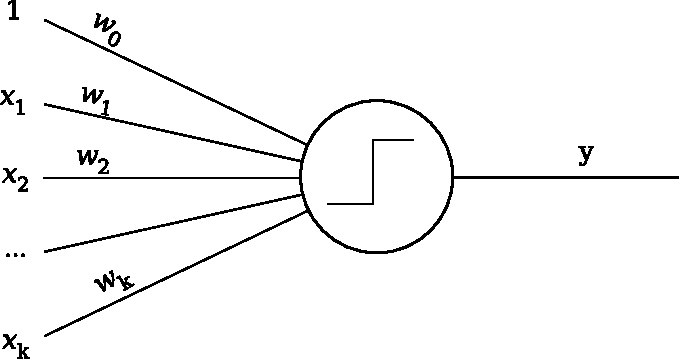
\includegraphics[scale=0.5]{perceptron.pdf}
        \end{center}
        \begin{enumerate}
            \item Implement a McCulloch-Pitts neuron (see the
                diagram):
                \begin{equation*}
                    y(\mathbf{x})=\sgn\left[
                    \mathbf{w}^T\mathbf{x}\right],
                \end{equation*}
                where $\mathbf{x}=[1, x_1, x_2,\dots, x_k]$ is a
                vector of inputs, $\mathbf{w}=[w_0, w_1, w_2, \dots,
                w_k]$ is a vector of weights and $y(\mathbf{x})$ is the
                output.
            \item Take weights $w=[-3, 2, 2]$ and two binary inputs
                $x_1, x_2 \in \{0, 1\}$. Show that the neuron performs a
            logical AND operation.
        \end{enumerate}
    \item \textbf{Rosenblatt's perceptron}
        \begin{enumerate}
            \item Prepare a training set $\left\{\mathbf{x}(i),
                d(\mathbf{x})\right\}$ for $i=1,2,\dots,n$, where
                $\mathbf{x}(i)=[1, x_1(i), x_2(i)]$ is the input
                vector and $d(\mathbf{x})$ is the desired response. Let the
                desired response be a comparison between two inputs:

                \begin{equation*}
                    d(\mathbf{x})=
                    \begin{cases}
                        1, & \text{if } x_1\geq x_2, \\
                        -1, & \text{if } x_1<x_2.
                    \end{cases}
                \end{equation*}
            \item Train a McCulloch-Pitts neuron on the training set
                using an error-correction update rule:
                \begin{equation}
                    \textbf{w}(k+1)=\mathbf{w}(k)+\eta
                    [d(k)-y(\mathbf{x}(k))]\mathbf{x}(k),
                    \label{eq:errorupdate}
                \end{equation}
                where $\eta>0$ is the learning rate.
                Present the training set repeatedly until no weight
                changes.
            \item Test on a new dataset (validation set) that the
                neuron can indeed perform the trained comparison function.
            \item\label{it:optimalweight} Plot the training set and label each
                input vector according to its response class. Superimpose the
                weight vector on the same plot (without bias term $w_0$).
                Explain why the weight vector is optimal.
            \item The expected probability of disagreement of a
                McCulloch-Pitts neuron and a goal function, which is
                implementable by this type of neuron, turns out to be
                proportional to the angle between the corresponding weights:
                \begin{equation}
                    \varepsilon_g(k) = \frac{1}{4} \left<
                    \left( y\left(\mathbf{x}\left(k\right)\right) -
                    d\left(\mathbf{x}\right) \right)^2 \right>_\mathbf{x} =
                    \frac{1}{\pi} \mathrm{arccos} \left( \frac{\mathbf{w}(k)
                    \cdot \mathbf{\tilde w}}{|\mathbf{w}(k)| |\mathbf{\tilde
                    w}|} \right),
                    \label{eq:generalizationerr}
                \end{equation}
                where $\mathbf{\tilde w}$ is the optimal weight vector
                from~\ref{it:optimalweight}. Study and plot the convergence
                behavior in time of the generalization error for the update
                rule in equation~\ref{eq:errorupdate}.
        \end{enumerate}
    \item \textbf{Linear separability}
        \begin{enumerate}
            \item Train a perceptron to perform the XOR function on binary
                inputs.
            \item Show that the learning algorithm does not converge
                i.e. the weights do not set to fixed values. What is the
                consequence for the generalization error of
                equation~\ref{eq:generalizationerr}?
            \item Plot the XOR classification problem on an
                Euclidean plane. Explain why the problem is not
                linearly separable. 
        \end{enumerate}

\end{enumerate}

\vfill
\centerline{\CAP Contact}
\CAP

\begin{tabular}{lll}
Urs Bergmann & Phone: 2093-8924 & Email:
urs.bergmann(at)biologie.hu-berlin.de \\
Matthias Guggenmos & & Email: matthias.guggenmos(at)bccn-berlin.de \\
Richard Kempter \hfill & Phone: 2093-8925 \hfill & Email:
r.kempter(at)biologie.hu-berlin.de \\
Robert Schmidt & Phone: 2093-8926 & Email: r.schmidt(at)biologie.hu-berlin.de
\\
Bartosz Telenczuk & Phone: 2093-8838 & Email:
b.telenczuk(at)biologie.hu-berlin.de \\
\end{tabular}

\end{document}
 
